\documentclass[default]{beamer}
\setbeamertemplate{navigation symbols}{}

\usetheme{CambridgeUS}
\useoutertheme{infolines}
%\usecolortheme{crane}

\usepackage{cmap}							% Поддержка поиска русских слов в PDF (pdflatex)
\usepackage[utf8]{inputenc}					% Выбор языка и кодировки
\usepackage[english, russian]{babel}
\usepackage{csquotes}

\usepackage[
	language=auto,
	autolang=other,
	backend=biber,
	style=authortitle,
	sorting=ydnt
]{biblatex}
\addbibresource{anokhin.bib}
				
\DeclareSourcemap{
	\maps[datatype=bibtex, overwrite]{
		\map{
			\step[fieldset=langid, fieldvalue=english]
			\step[fieldset=doi, null]
			\step[fieldset=issn, null]
			\step[fieldset=isbn, null]
			\step[fieldset=url, null]
			\step[fieldsource=language, fieldset=langid, origfieldval]
		}
	}
}


\graphicspath{{../../images/cognitome/}} 			% Пути к изображениям

\makeatletter
\setbeamertemplate{footline}
{
	\leavevmode%
	\hbox{%
		\begin{beamercolorbox}[wd=.333333\paperwidth,ht=2.25ex,dp=1ex,center]{author
				in head/foot}%
			\usebeamerfont{author in
				head/foot}\insertshortauthor~~\beamer@ifempty{\insertshortinstitute}{}{(\insertshortinstitute)}
		\end{beamercolorbox}%
		\begin{beamercolorbox}[wd=.333333\paperwidth,ht=2.25ex,dp=1ex,center]{title in
				head/foot}%
			\usebeamerfont{title in head/foot}\insertshorttitle
		\end{beamercolorbox}%
		\begin{beamercolorbox}[wd=.333333\paperwidth,ht=2.25ex,dp=1ex,right]{date in
				head/foot}%
			\usebeamerfont{date in head/foot}\insertshortdate{}\hspace*{2em}
			\insertframenumber{}\hspace*{2ex} 
		\end{beamercolorbox}
	}%
	\vskip0pt%
}


\renewcommand*{\bibfont}{\tiny}
\setlength\bibitemsep{-5pt}

\begin{document}
	
	\title[Cognitome]{Теория когнитома Анохина}
	\author[Панов]{Александр Панов}
	\institute[ИСА РАН]{ИСА РАН}
	\date{1 июня 2016~г.} 
	
	\begin{frame}
		\titlepage
	\end{frame}
		
	\begin{frame}
		\frametitle{Константин Владимирович Анохин}
		
		\footnotesize
		\begin{columns}
			\begin{column}{0.8\textwidth}
				\begin{itemize}
					\item Константин Владимирович Анохин "--- нейробиолог, специалист в области молекулярной биологии, исследования памяти.
					\item Член-корреспондент РАН и РАМН, руководитель отдела нейронаук НИЦ <<Курчатовский институт>>.
					\item \href{https://www.scopus.com/authid/detail.uri?authorId=7004196582}{Scopus}: 146 статей, 1185 цитирований, h-индекс "--- 17.
					\item \href{http://elibrary.ru/author_items.asp?authorid=692}{РИНЦ}: 177 статей, 1588 цитирований, h-индекс "--- 18.
				\end{itemize}
			\end{column}
			\begin{column}{0.2\textwidth}
				\begin{figure}
					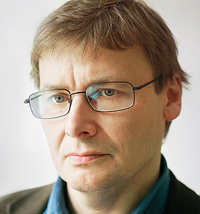
\includegraphics[width=\textwidth]{anokhin}
				\end{figure}
			\end{column}
		\end{columns}
		\par\medskip
		\textbf{Основные публикации:}
		\nocite{*}
		\printbibliography
	\end{frame}
	

	\begin{frame}	
		\frametitle{Когнитивные вычисления}
		
		\begin{itemize}
			\item IBM - Cognitive Computing 2006, Cognitive Computing via Synaptronics and Supercomputing (C2S2).
			\item DARPA - развить нейроморфные машины до биологического уровня.
			\item SyNAPSE - Systems of Neuromorphic Adaptive Plastic Scalable Electronics.
		\end{itemize}
		
	\end{frame}	

	\begin{frame}
		\frametitle{Кортикоморфные когнитивные архитектуры}
		
		\begin{itemize}
			\item Кортикальный вычислительынй примитив (cortical computing primitive) - определенная области неокортекса, выполняет <<стандартные>> операции и объединяется в большие сети для выполнения высокоуровневых функций.
			\item Реккурентные нейронные цепи являются прообразами таких примитивов: состоят из 100--10000 нейронов, около 50-1000 микрон в диаметре.
		\end{itemize}
		
		\begin{figure}
			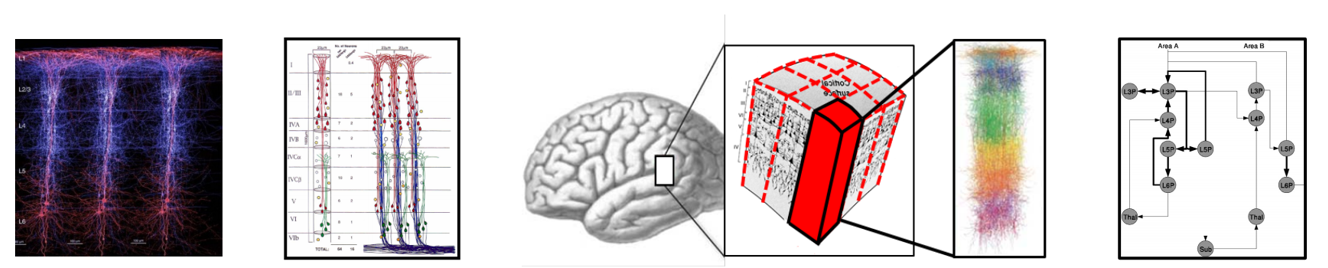
\includegraphics[width=\textwidth]{brain-prim}
		\end{figure}
		
	\end{frame}	
	
	\begin{frame}	
		\frametitle{Кортикоморфные когнитивные архитектуры}
		
		\begin{itemize}
			\item Реконструировать кортикальные нейронные цепи для определения кортикального вычислительного примитива: идентификация их структуры, функций и параметров с помощью инструментов картирования мозга, получение результата в виде аттрибутированного графа или аннотированной схемы.
			\item Идентифицировать функции (примитивы), выполняемые этими цепями.
			\item Использовать примитивы как строительные блоки для разработки новых алгоритмов машинного обучения.
		\end{itemize}
		
		\begin{figure}
			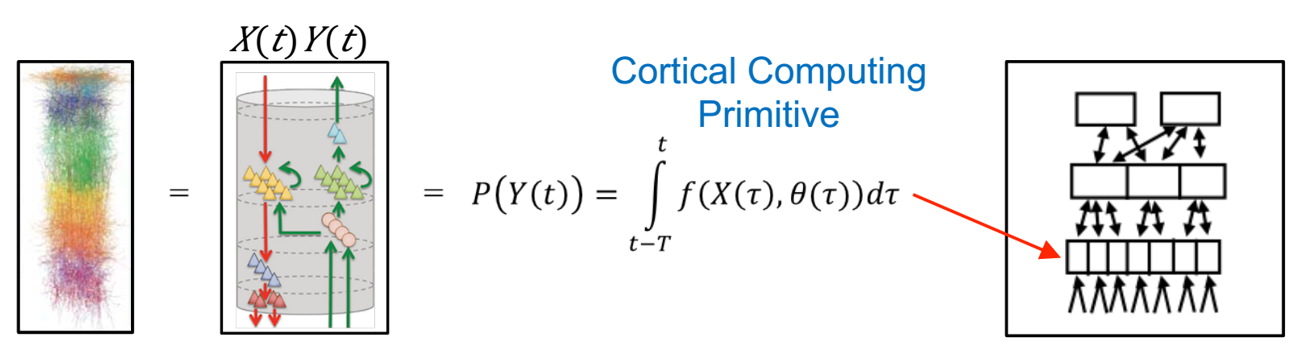
\includegraphics[width=0.8\textwidth]{cortic-morph}
		\end{figure}
		
	\end{frame}		
	
	\begin{frame}
		\frametitle{Кортикоморфные когнитивные архитектуры}
		
		\begin{figure}
			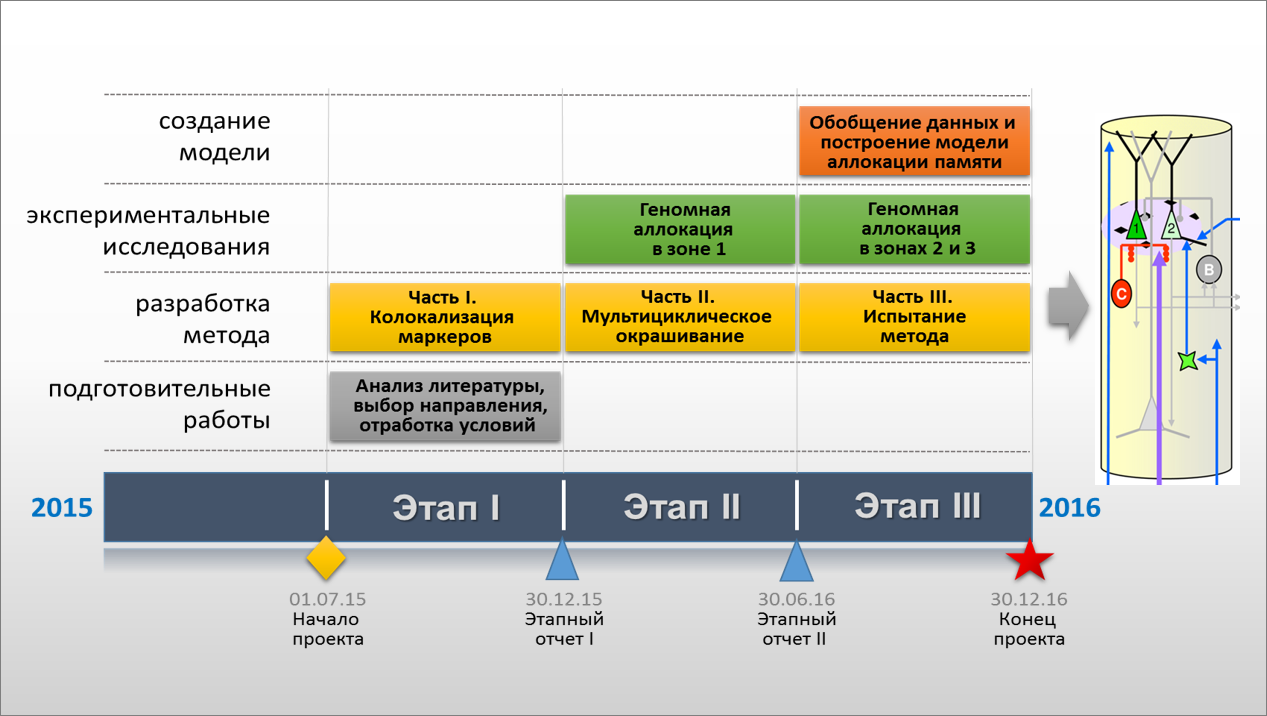
\includegraphics[width=\textwidth]{minobr_proj}
		\end{figure}
	\end{frame}	

	\begin{frame}
		\frametitle{Кортикоморфные когнитивные архитектуры}
		
		\begin{figure}
			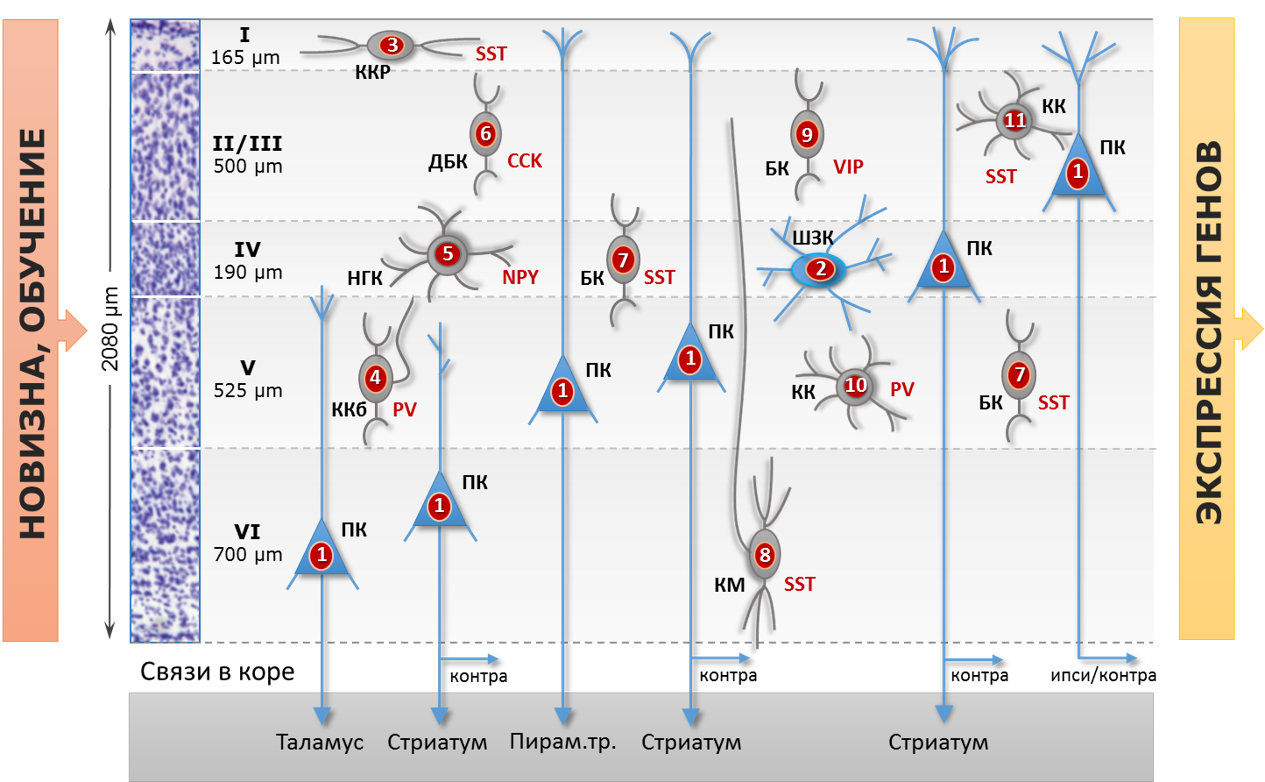
\includegraphics[width=\textwidth]{info_allocat}
		\end{figure}
	\end{frame}	

	\begin{frame}	
		\frametitle{Сети - это важно}

		\begin{columns}
			\begin{column}{0.3\textwidth}		
				\begin{figure}
					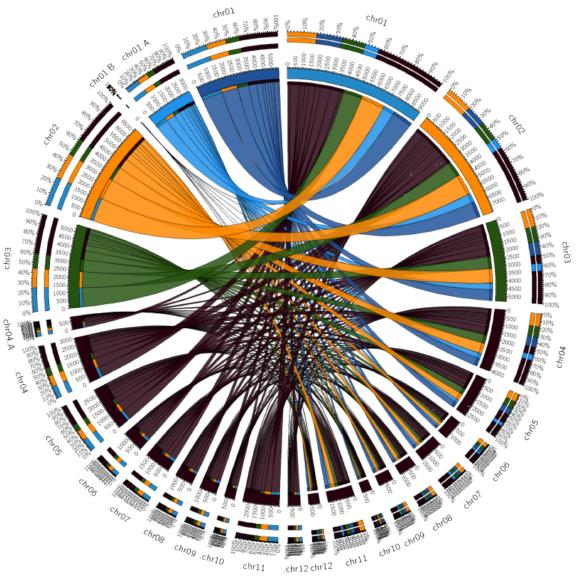
\includegraphics[width=\textwidth]{genome}
				\end{figure}
				\centering
				Геном
			\end{column}
			\begin{column}{0.3\textwidth}		
				\begin{figure}
					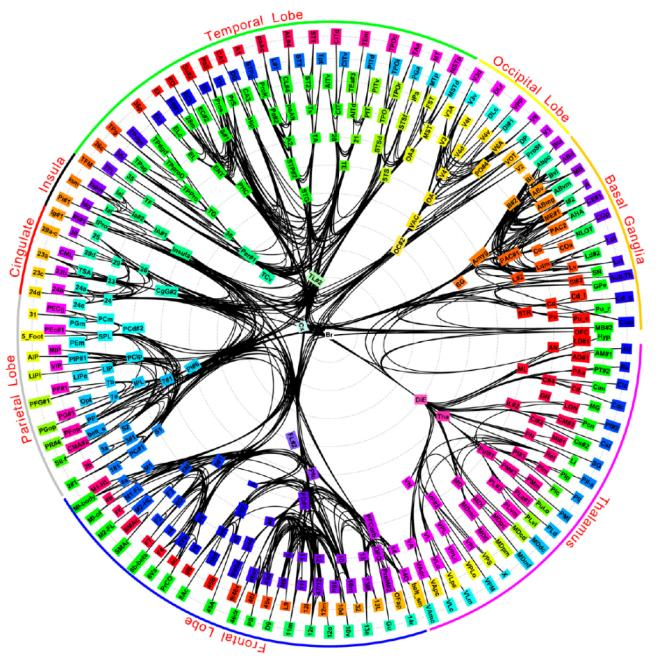
\includegraphics[width=\textwidth]{connectome}
				\end{figure}
				\centering
				Коннектом
			\end{column}
			\begin{column}{0.3\textwidth}		
				\begin{figure}
					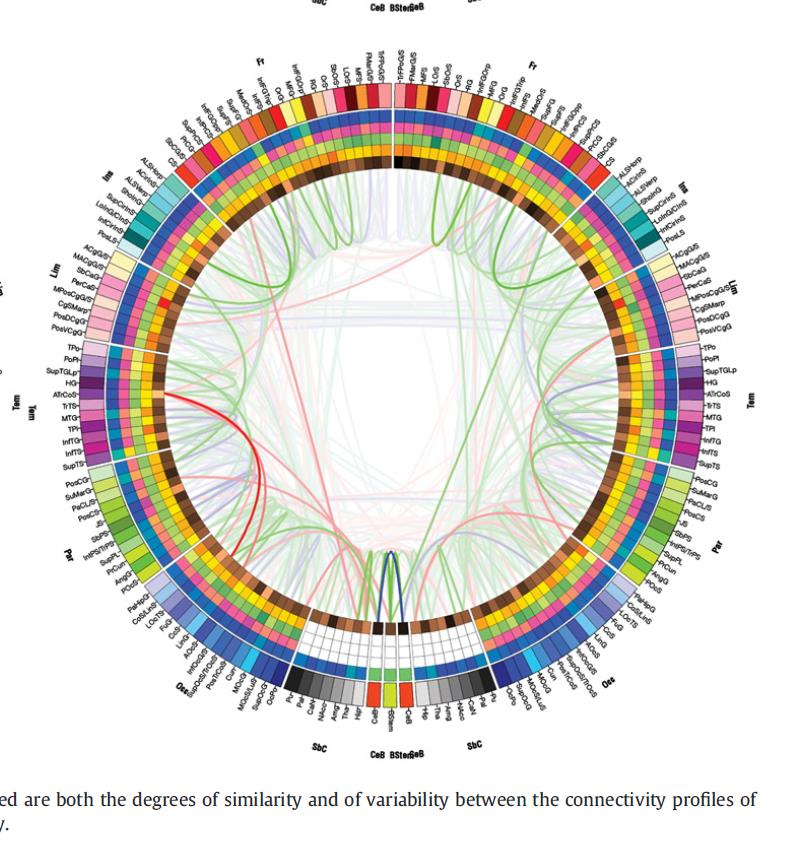
\includegraphics[width=\textwidth]{cognitome}
				\end{figure}
				\centering
				Когнитом
			\end{column}
		\end{columns}		
	\end{frame}
	
	\begin{frame}
		\frametitle{Нейронные гиперсети}
		
		\begin{figure}
			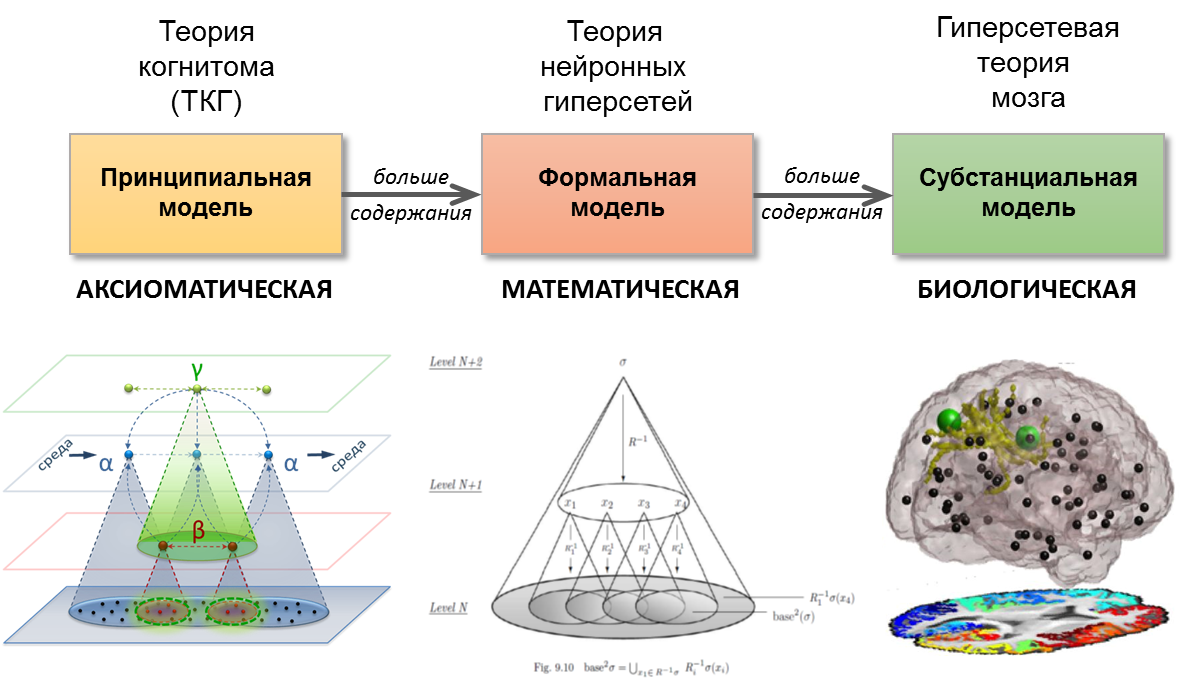
\includegraphics[width=\textwidth]{etaps}
		\end{figure}
	\end{frame}	
															
	\begin{frame}
		\frametitle{Нейронные гиперсети}
		
		\begin{figure}
			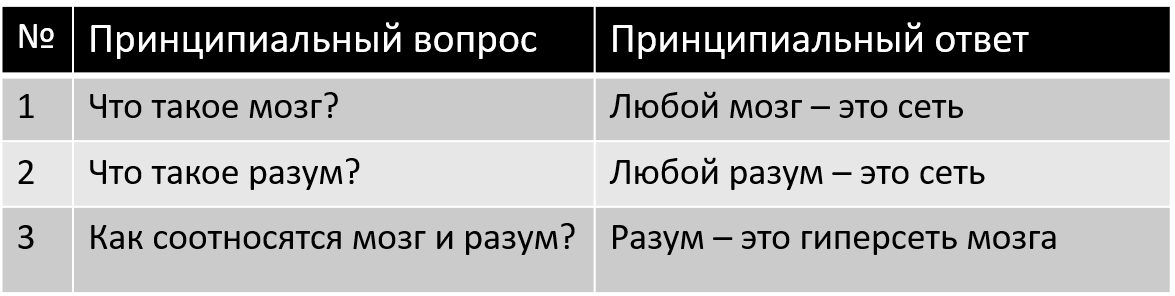
\includegraphics[width=\textwidth]{quest-answer}
		\end{figure}
		\begin{columns}
			\begin{column}{0.3\textwidth}
				\begin{figure}
					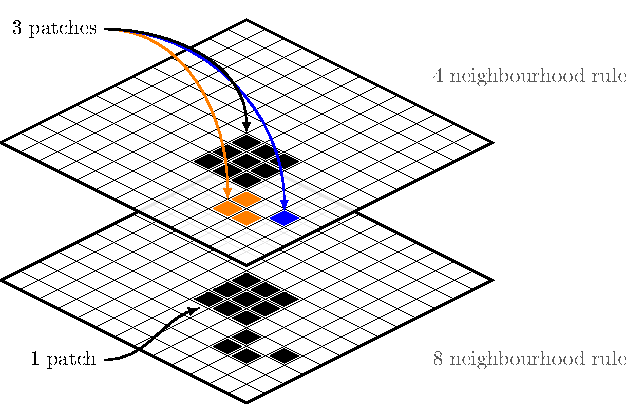
\includegraphics[width=\textwidth]{layers}
				\end{figure}
			\end{column}
			\begin{column}{0.7\textwidth}
				\begin{itemize}
					\item Разум – это \textbf{структура}.
					\item Разум – это \textbf{многослойная} макроструктура мозга: сеть сетей нейрональных сетей.
					\item Мышление и сознание – это особые виды \textbf{траффика} в этой макроструктуре.
				\end{itemize}
			\end{column}
		\end{columns}
	\end{frame}	
	
	\begin{frame}
		\frametitle{Что нужно, чтобы возник когнитивный агент?}
		
		Теория утверждает, что существует три необходимых и достаточных условия для возникновения разумного (интеллектуального, когнитивного) агента:
		\begin{itemize}
			\item адаптивный агент должен состоять из \textbf{функциональных систем} (ФС);
			\item функциональные системы должны занимать \textbf{нервную сеть} (НС);
			\item нервная сеть должна иметь механизмы \textbf{долговременной памяти} (ДП).
		\end{itemize}
		\par\bigskip
		Разум будет эволюционно возникать в любом адаптивном агенте, имеющем эти три условия.
	\end{frame}
			
	\begin{frame}
		\frametitle{Разум как макросистема мозга}

		Разум \textbf{реален} – он образует макросистемный уровень когнитивного агента, опосредующий его информационные соотношения со средой. 
				
		\begin{figure}
			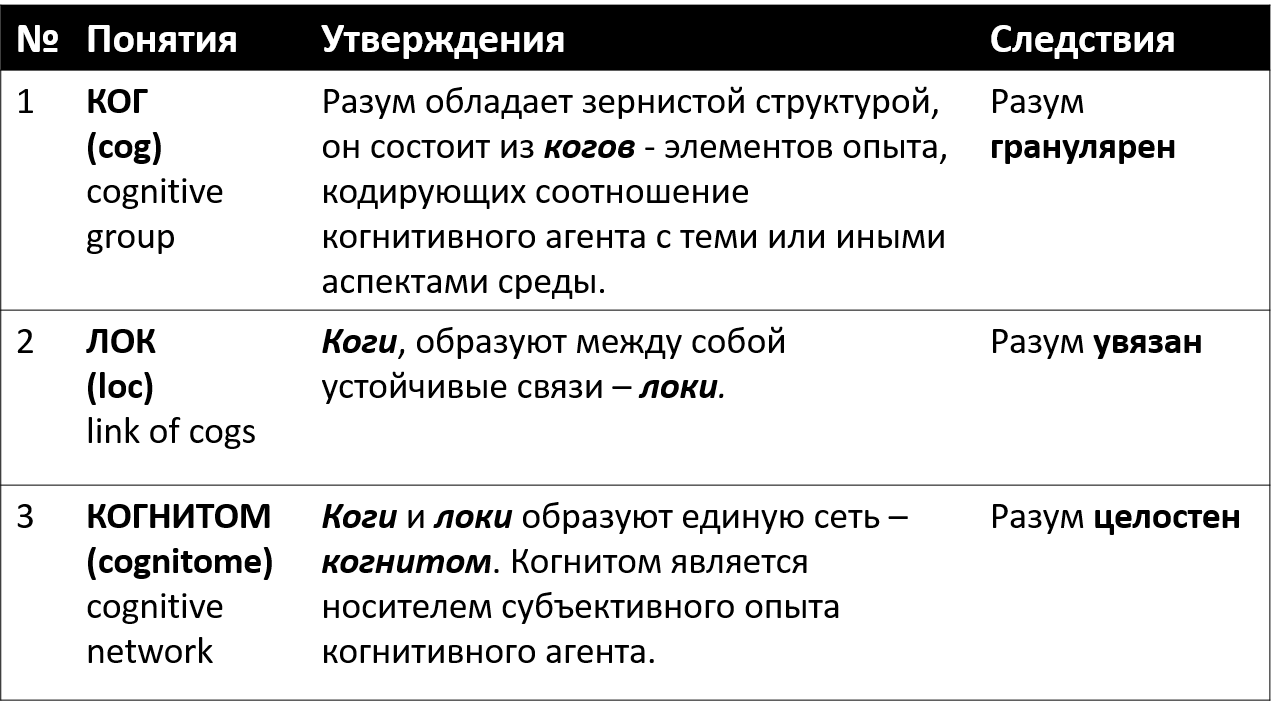
\includegraphics[width=0.8\textwidth]{concepts}
		\end{figure}
	\end{frame}	

	\begin{frame}
		\frametitle{Ког и когнитом}
		
		Ког – когнитивная группа.
		
		\begin{columns}
			\begin{column}{0.3\textwidth}
				\begin{figure}
					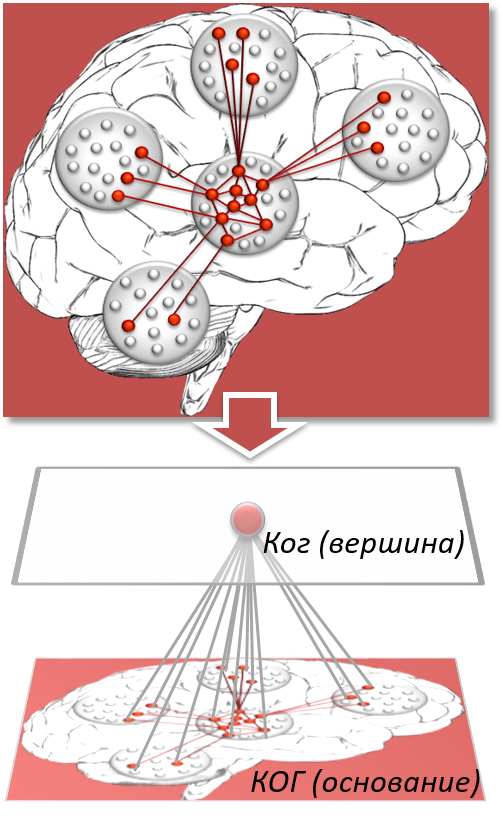
\includegraphics[width=\textwidth]{cog}
				\end{figure}
			\end{column}
			\begin{column}{0.7\textwidth}
				\textbf{Ког} - распределенная группа нейронов, сцепленная единым когнитивным опытом.  
				\par\bigskip
				\textbf{Когнитом}  –  сеть из всех когнитивных элементов (КОГов)  в нервной системе адаптивного агента.
			\end{column}
		\end{columns}
	\end{frame}

	\begin{frame}
		\frametitle{Ког - сноп}
		
		\begin{figure}
			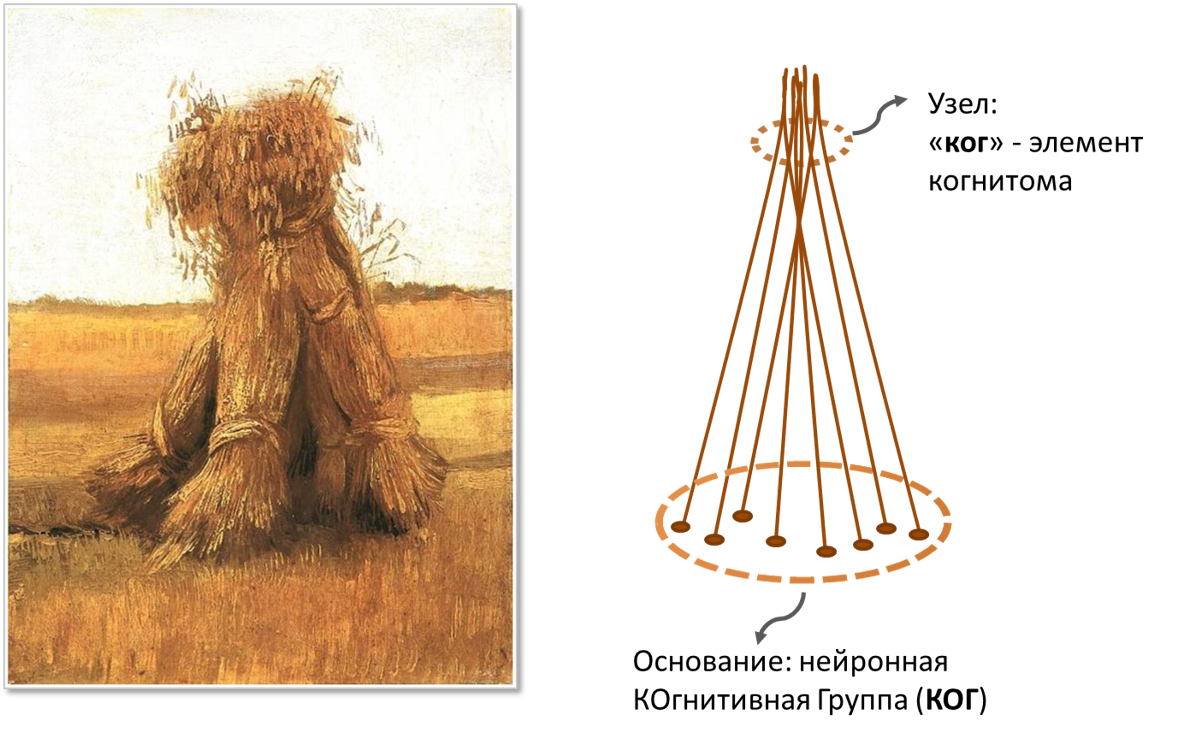
\includegraphics[width=\textwidth]{stog}
		\end{figure}
	\end{frame}

	\begin{frame}
		\frametitle{Ког - гиперсимплекс в гиперсети}
		\footnotesize
		\begin{itemize}
			\item Гиперсети состоят из геометрических структур, известных как гиперсимплексы.
			\item Основание гиперсимплекса содержит множество элементов одного уровня, а его вершина образуется описанием их отношений и приобретает интегральные свойства, делающие ее элементом сети более высокого уровня – гиперсети.
			\item Гиперсеть представляет собой совокупность связанных гиперсимплексов. 
			\item Гиперсети являются инструментом формализации структуры и динамики в многоуровневых системах.
		\end{itemize}
		\begin{figure}
			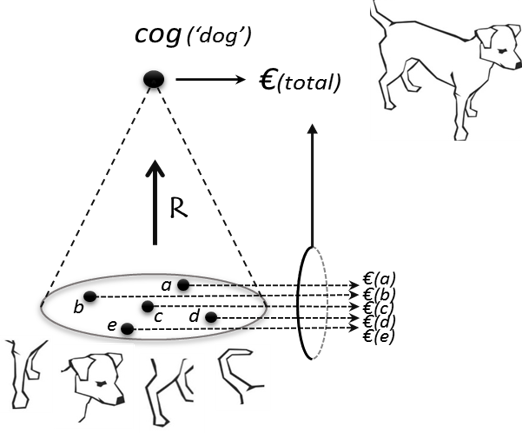
\includegraphics[width=0.4\textwidth]{cog-dog}
		\end{figure}
	\end{frame}	
	
	\begin{frame}
		\frametitle{Гиперсети}
		
		Гиперсети характеризуются тремя основными идеями: 
		\begin{enumerate}
			\item «реляционного симплекса» или «гиперсимплекса», 
			\item того, что гиперсимплексы являются однозначным средством различения уровней в многоуровневых системах и 
			\item того, что они могут поддерживать устойчивую структуру (backcloth) и динамику активности (traffic) в многоуровневых системах.
		\end{enumerate}
		
		\begin{figure}
			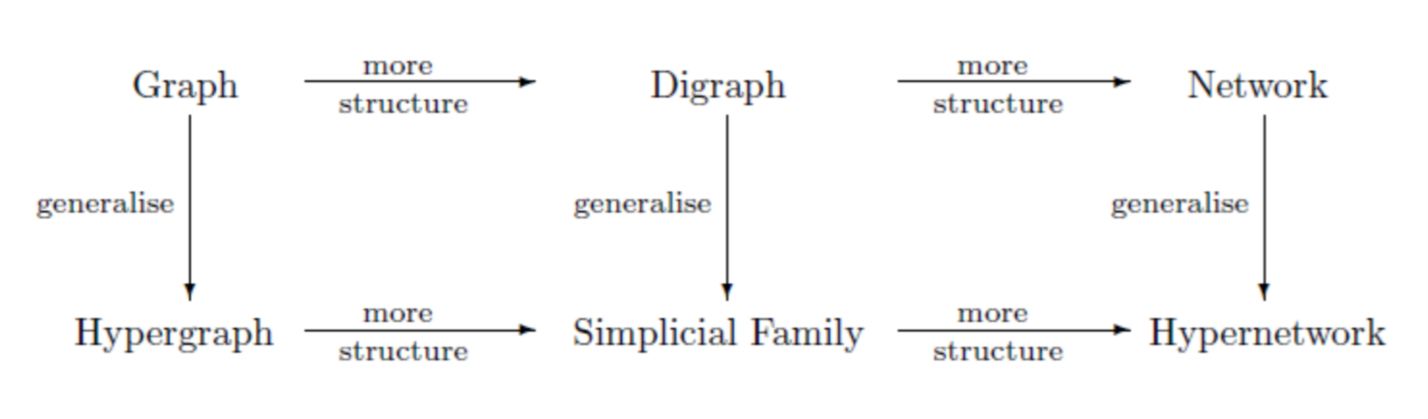
\includegraphics[width=\textwidth]{gipergraph}
		\end{figure}
	\end{frame}	
		
	\begin{frame}	
		\frametitle{Гиперсети}
		
		\begin{figure}
			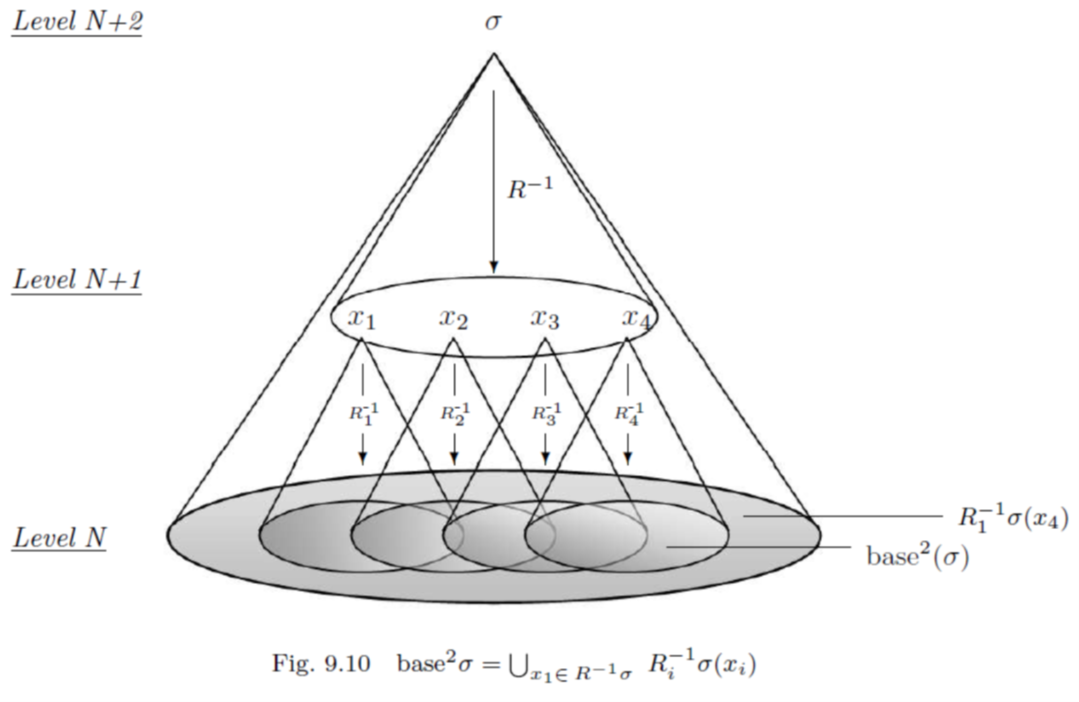
\includegraphics[width=0.8\textwidth]{gipergraph2}
		\end{figure}
	\end{frame}
	
	\begin{frame}	
		\frametitle{Три принципа генерации когов}
		
		\begin{figure}
			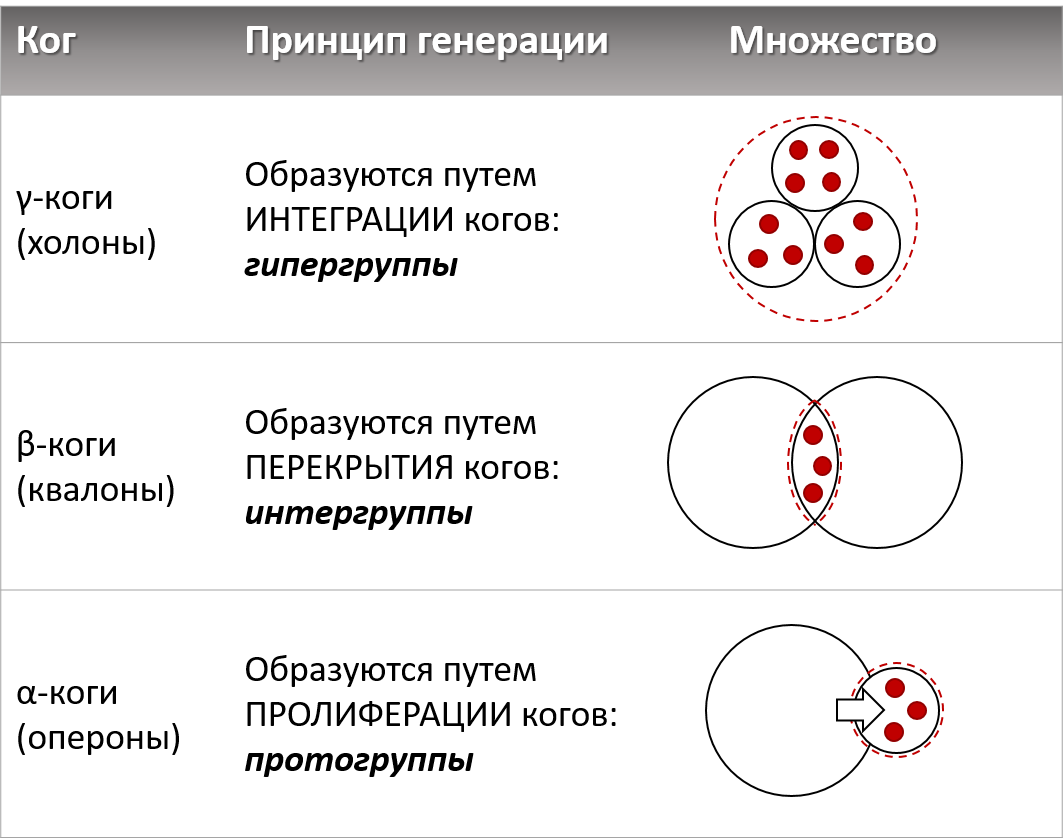
\includegraphics[width=0.7\textwidth]{cog-types}
		\end{figure}
	\end{frame}

	\begin{frame}
		\frametitle{Три слоя когнитивной сети мозга}
		
		Любой когнитивный агент имеет два макроуровня в организации своей нервной сети:
		\begin{itemize}
			\item Сеть из функциональных систем ($\alpha$-когнитивные группы и их связи)
			\item Сеть из метасистемных модулей ($\beta$-когнитивные группы и их связи)
		\end{itemize}
		\par\bigskip
		Когнитивный агент может также иметь третью - факультативную сеть:
		\begin{itemize}
			\item Сеть из гиперсистемных комплексов ($\gamma$-когнитивные группы и их связи)
		\end{itemize}
		\par\bigskip
		\textbf{$\alpha$- и $\beta$- сети обусловливают ПСИХИКУ когнитивного агента, а $\gamma$- сеть обусловливает СОЗНАНИЕ когнитивного агента.}
	\end{frame}

	\begin{frame}	
		\frametitle{$\alpha$-коги}
		
		$\alpha$-коги – это классические функциональные системы, обладают операциональной архитектоникой
		и выделяются по результату для адаптивного агента, имеют распределенную локализацию в мозге, образуют связи друг с другом - $\alpha$-локи.
		
		\begin{figure}
			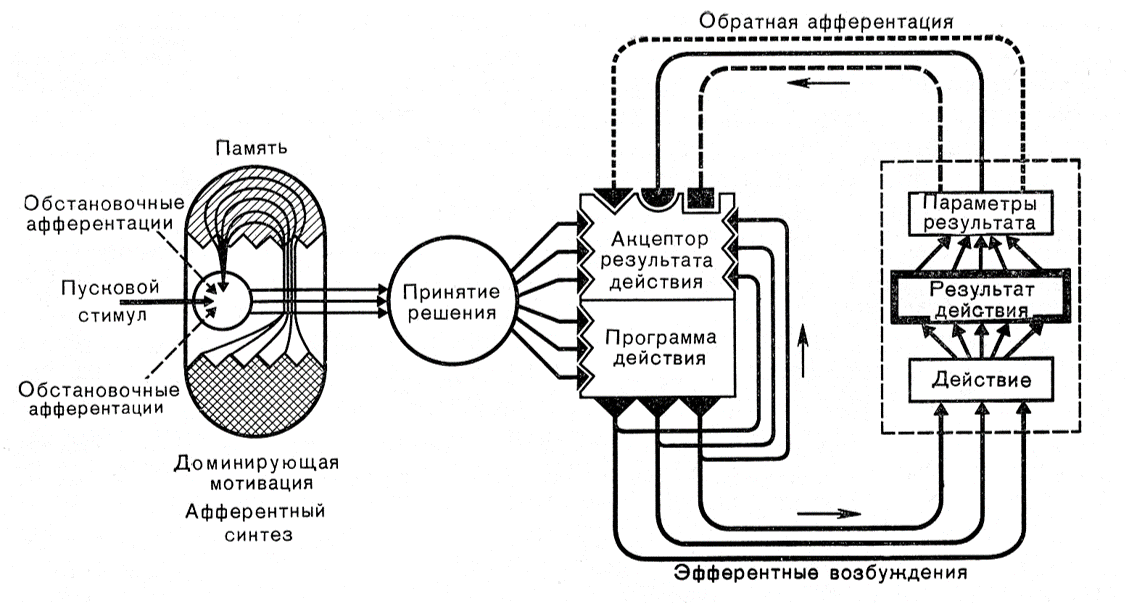
\includegraphics[width=0.7\textwidth]{func_system}
		\end{figure}
	\end{frame}		
	
	\begin{frame}	
		\frametitle{$\beta$-коги}
		
		$\beta$-коги – это классические нейронные ансамбли.
		
		\begin{figure}
			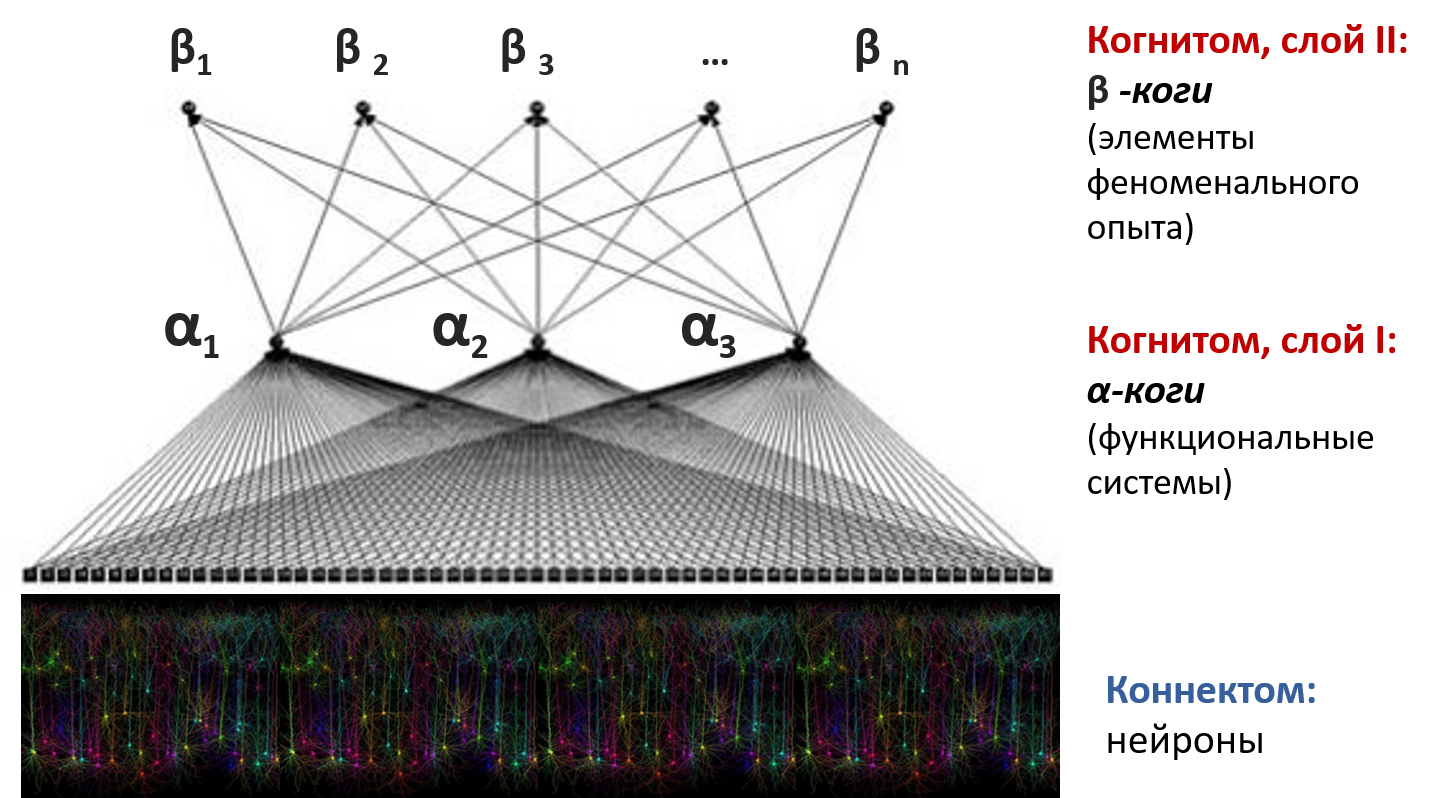
\includegraphics[width=\textwidth]{beta-cog}
		\end{figure}
	\end{frame}	
	
	\begin{frame}	
		\frametitle{$\gamma$-коги}

		\begin{figure}
			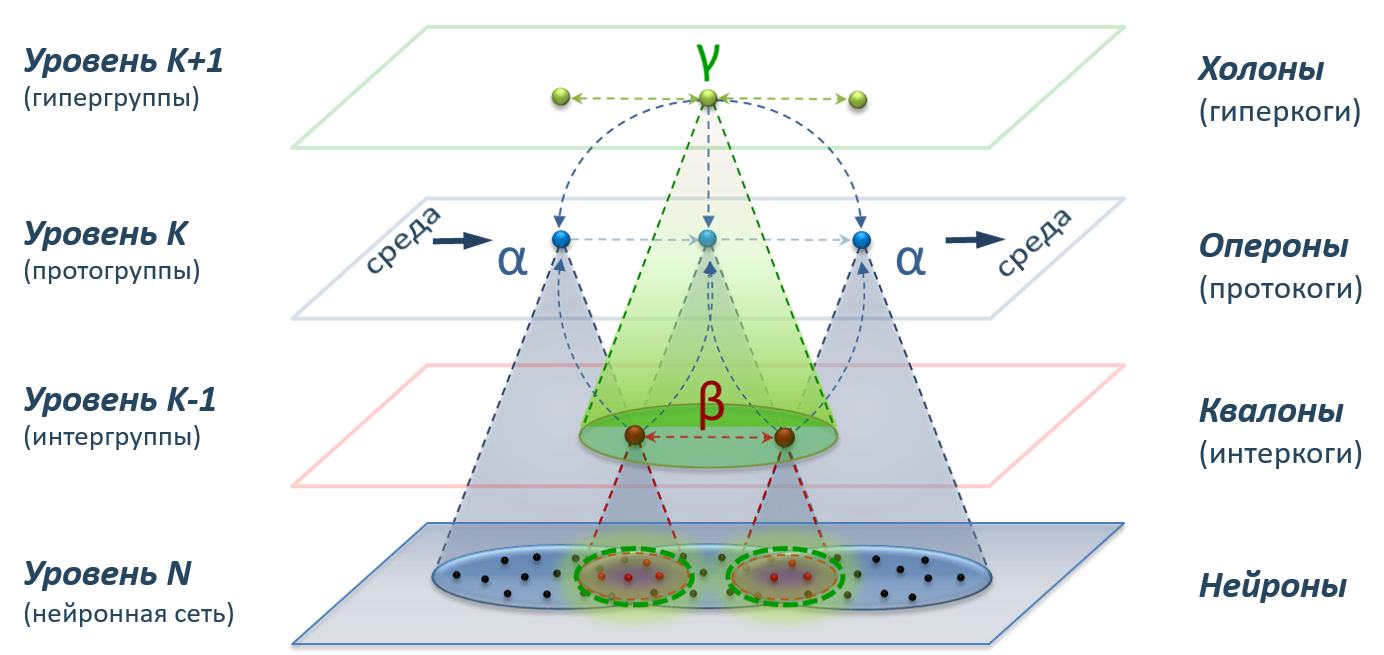
\includegraphics[width=\textwidth]{gamma-cog}
		\end{figure}
		
		Трехслойная структура когнитома обеспечивает «дискретную бесконечность» и одновременно целостность психики и сознания.
		
	\end{frame}		
	
	\begin{frame}	
		\frametitle{Призывы}
		
		\begin{itemize}
			\item Нам нужна третья революция в области когнитивной науки.
			\item Нам нужны принципиально новые идеи для создания искусственных когнитивных систем и когнитивных вычислений.
		\end{itemize}
		
	\end{frame}	
												
%	\begin{frame}
%		\frametitle{Цели курса}
%		
%		\begin{columns}
%			\begin{column}{0.5\textwidth}
%				
%			\end{column}
%			\begin{column}{0.5\textwidth}
%				\begin{figure}
%					
\includegraphics[width=\textwidth]{logo}
%				\end{figure}
%			\end{column}
%		\end{columns}
%	\end{frame}
	%	\begin{frame}
	%		\frametitle{Цели курса}
	%		
	%		\begin{itemize}
	%			\item
	%		\end{itemize}
	%	\end{frame}
	
\end{document}
	
	
